\documentclass[aspectratio=169]{beamer}
\usetheme{Madrid}
\usecolortheme{seahorse}

\usepackage[utf8]{inputenc}
\usepackage{graphicx}
\usepackage{booktabs}
\usepackage{tikz}
\usetikzlibrary{shapes.geometric, arrows.meta, positioning, calc, fit}

\title[Nepali Search Prototype]{Minimalistic Nepali Search Engine Prototype}
\subtitle{Hybrid IR Architecture \& Local RAG Pipeline}
\author[Sujal Bajracharya]{Sujal Bajracharya}
\institute[KU]{Kathmandu University}
\date{\today}

\begin{document}

% Slide 1: Title
\begin{frame}
  \titlepage
\end{frame}

% Slide 2: Task Assigned & Objective
\begin{frame}{Task Assigned \& Project Goal}
  \begin{block}{Assigned Task}
    \textbf{Task 3:} Research and develop a \textbf{Minimalistic Nepali Search Engine Prototype}.
  \end{block}
  \vspace{0.3cm}
  \begin{itemize}
    \item \textbf{Core Goal:} Validate end-to-end search mechanics (indexing, retrieval, fusion, and answer generation) for Devanagari text.
    \item \textbf{Complementary Scope:} Operates as an engineering sandbox while teammates (Aarav \& Shova) build standard traditional and RAG IR benchmark datasets.
    \item \textbf{Primary Deliverable:} A working full-stack prototype (FastAPI + React) powered by a hybrid sparse-dense retriever and a RAG pipeline.
  \end{itemize}
\end{frame}

% Slide 3: Outline
\begin{frame}{Presentation Outline}
  \tableofcontents
\end{frame}

% Slide 4: The Datasets
\section{Dataset Selection}
\begin{frame}{Dataset Selection \& Strategy}
  \begin{columns}
    \column{0.5\textwidth}
    \begin{block}{Evaluated Datasets}
      \begin{itemize}
        \item \textbf{Nepali Wikipedia Dump:} $\sim$31k clean articles, highly factual but rigid vocabulary.
        \item \textbf{Nepali News Corpus (\texttt{spandyie}):} $\sim$2.76M articles with headlines, bodies, and categories.
      \end{itemize}
    \end{block}
    
    \column{0.5\textwidth}
    \begin{block}{Choice: Nepali News Corpus}
      \begin{itemize}
        \item Realistic user search queries mirror news headlines.
        \item Varied article lengths for testing length normalization ($b$ in BM25).
      \end{itemize}
    \end{block}
  \end{columns}
  
  \vspace{0.4cm}
  \begin{alertblock}{Important Development Note}
    Currently used strictly as an \textbf{indexing corpus}. It lacks query-relevance pairs ($qrels$), which are currently being developed by the benchmark team.
  \end{alertblock}
\end{frame}

% Slide 5A: Enterprise Search Servers
\begin{frame}{Framework Analysis: Enterprise Search Servers}
  \begin{block}{How Elasticsearch \& Apache Solr Work}
    Standalone server processes built on Apache Lucene. They expose HTTP REST or XML APIs and manage distributed inverted indexes, sharding, and cluster state.
  \end{block}
  
  \vspace{0.2cm}
  \begin{columns}
    \column{0.5\textwidth}
    \begin{exampleblock}{Key Strengths}
      \begin{itemize}
        \item High horizontal scaling for web production.
        \item Robust multi-tenant query management.
      \end{itemize}
    \end{exampleblock}
    
    \column{0.5\textwidth}
    \begin{alertblock}{Why They Fail for Nepali Sandbox}
      \begin{itemize}
        \item \textbf{High Overhead:} Massive JVM resource footprint for a research environment.
        \item \textbf{Devanagari Pipeline Friction:} Custom stemming rules require compiling and deploying custom Java plugins.
      \end{itemize}
    \end{alertblock}
  \end{columns}
\end{frame}

% Slide 5B: Native Libraries & Vector Databases
\begin{frame}{Framework Analysis: Core Libraries \& Vector DBs}
  \begin{columns}
    \column{0.5\textwidth}
    \begin{block}{Apache Lucene (Core Java)}
      \begin{itemize}
        \item \textbf{Mechanism:} Low-level Java library that constructs inverted posting lists for term frequency scoring (BM25).
        \item \textbf{Limitation:} Lacks a direct Python API. Calling it natively requires complex Java Native Interface (JNI) bindings.
      \end{itemize}
    \end{block}

    \column{0.5\textwidth}
    \begin{block}{FAISS (C++ / Python)}
      \begin{itemize}
        \item \textbf{Mechanism:} Dense vector library optimizing Approximate Nearest Neighbor (ANN) search via HNSW graphs or IVF vector quantization.
        \item \textbf{Limitation:} Zero sparse/keyword search capability; requires external text-to-ID mapping.
      \end{itemize}
    \end{block}
  \end{columns}

  \vspace{0.3cm}
  \begin{alertblock}{The Integration Bottleneck}
    Combining Lucene and FAISS manually requires writing custom synchronization scripts to keep document internal IDs aligned across two separate indexes.
  \end{alertblock}
\end{frame}

% Slide 5C: The Winning Architecture - Pyserini
\begin{frame}{Why Pyserini is the Optimal Fit for Nepali IR}
  \begin{block}{How Pyserini Works}
    A Python IR toolkit that uses Py4J to bridge Python directly to Java Lucene for sparse BM25 indexing, while integrating directly with C++/Python FAISS for dense vector indexing.
  \end{block}

  \vspace{0.2cm}
  \begin{block}{Key Architectural Advantages for Devanagari}
    \begin{itemize}
      \item \textbf{Bypasses Java Analyzer Constraints:} Allows Python pre-tokenization (`unicodedata`, `nepalikit`) passed directly via Lucene’s `JWhiteSpaceAnalyzer`.
      \item \textbf{Native PyTorch / HuggingFace Integration:} Runs neural embeddings (`multilingual-e5-large`) in the same Python runtime as sparse indexes.
      \item \textbf{Automated ID Sync \& Fusion:} The `HybridSearcher` class natively maps Lucene and FAISS docIDs and executes Reciprocal Rank Fusion (RRF) in memory.
    \end{itemize}
  \end{block}
\end{frame}

% Slide 6: Why Pyserini
\begin{frame}{Why Pyserini for BM25 \& Vector Search?}
  \begin{block}{Why Not FAISS Alone?}
    \begin{itemize}
      \item FAISS is strictly a vector index—it cannot perform BM25 keyword matching or document management.
      \item Running raw Lucene + FAISS separately requires \textbf{manual document ID synchronization} and custom fusion scripts.
    \end{itemize}
  \end{block}
  \vspace{0.2cm}
  \begin{block}{The Pyserini Advantage}
    \begin{itemize}
      \item Wraps both \textbf{Lucene} (Sparse BM25) and \textbf{FAISS} (Dense Vectors) into a single Python interface.
      \item Native \texttt{HybridSearcher} class automatically manages ID alignment and executes \textbf{Reciprocal Rank Fusion (RRF)}.
    \end{itemize}
  \end{block}
\end{frame}

% Slide 7: Preprocessing Pipeline with Libraries
\section{Text Preprocessing}
\begin{frame}{Devanagari Preprocessing Pipeline \& Libraries}
  \begin{enumerate}
    \item \textbf{Unicode Normalization (NFKC):} Unifies Devanagari codepoints and strips zero-width joiners (\texttt{\textbackslash u200d}). \\
          $\rightarrow$ \textbf{Library:} Python \texttt{unicodedata}
    \item \textbf{Noise \& Symbol Stripping:} Removes HTML tags, non-Devanagari symbols, and punctuation. \\
          $\rightarrow$ \textbf{Library:} Python \texttt{re} (Regular Expressions) / \texttt{nepalikit}
    \item \textbf{Rule-Based Suffix Stripping:} Strips attached postpositions (\textit{-हरूबाट}, \textit{-मा}, \textit{-को}, \textit{-का}, \textit{-सँग}, \textit{-ले}, \textit{-लाई}). \\
          $\rightarrow$ \textbf{Library:} Custom Regex Rules / \texttt{nepali-stemmer}
    \item \textbf{Stopword Filtering:} Drops high-frequency functional words (\textit{र}, \textit{छ}, \textit{हो}, \textit{भने}, \textit{पनि}). \\
          $\rightarrow$ \textbf{Library:} \texttt{nepalikit} / Custom set
    \item \textbf{Token Reassembly \& Ingestion:} Space-separated string passed to Lucene's \texttt{JWhiteSpaceAnalyzer}. \\
          $\rightarrow$ \textbf{Library:} \texttt{pyserini}
  \end{enumerate}
\end{frame}

% Slide 8: BM25 Indexing
\begin{frame}{BM25 Indexing via Pyserini}
  \begin{block}{Pre-tokenized Whitespace Strategy}
    Instead of relying on Lucene's default analyzer, we pass space-separated, pre-stemmed tokens to Pyserini using Lucene's \texttt{JWhiteSpaceAnalyzer}.
  \end{block}
  \vspace{0.3cm}
  \textbf{Corpus Ingestion Format (\texttt{.jsonl}):}
  \begin{exampleblock}{JSONL Payload}
    \texttt{\{"id": "doc\_001", "contents": "काठमाडौँ मानिस घर बाहिर निस्किए"\}}
  \end{exampleblock}
  \vspace{0.2cm}
  \textbf{Pyserini Command:} \\
  \texttt{\small python -m pyserini.index.lucene --collection JsonCollection --input corpus/ --index index/ --generator DefaultLuceneDocumentGenerator --threads 4 --stemmer none --keepStopwords --analyzer JWhiteSpaceAnalyzer}
\end{frame}

% Slide 9: Neural Encoders
\section{Neural Retrieval}
\begin{frame}{Neural Encoder: \texttt{multilingual-e5-large}}
  \begin{columns}
    \column{0.6\textwidth}
    \begin{itemize}
      \item \textbf{Foundation:} Fine-tuned from Facebook AI's \textbf{XLM-RoBERTa Large}.
      \item \textbf{Embedding Size:} 1024-dimensional dense vectors.
      \item \textbf{Multilingual Strength:} Strong cross-lingual mapping for Devanagari script.
    \end{itemize}
    
    \column{0.4\textwidth}
    \begin{alertblock}{Asymmetric Prefixes}
      Must append prefixes for accurate dense retrieval:
      \begin{itemize}
        \item Documents: \texttt{"passage: "}
        \item Queries: \texttt{"query: "}
      \end{itemize}
    \end{alertblock}
  \end{columns}
\end{frame}

% Slide 10: Hybrid Integration
\begin{frame}{Integrating Hybrid Search in Pyserini}
  \begin{block}{Hybrid Searcher Execution}
    Pyserini combines BM25 scores and Dense E5 embeddings using \textbf{Reciprocal Rank Fusion (RRF)}:
    $$RRF\_Score(d) = \sum_{m \in M} \frac{1}{k + r_m(d)}$$
    \textit{where $k=60$, and $r_m(d)$ is the document rank in retriever $m$.}
  \end{block}
  \vspace{0.3cm}
  \begin{exampleblock}{Python Implementation}
    \texttt{from pyserini.search.hybrid import HybridSearcher}\\
    \texttt{searcher = HybridSearcher(dense\_searcher, sparse\_searcher)}\\
    \texttt{hits = searcher.search(query, k=10, rrf\_k=60)}
  \end{exampleblock}
\end{frame}

% Slide 11: RAG LLMs
\section{RAG Integration}
\begin{frame}{RAG Generation: Available LLM Options}
  \begin{columns}
    \column{0.5\textwidth}
    \begin{block}{Local GPU Execution}
      \textbf{\texttt{Llama-3.2-3B-Instruct}}
      \begin{itemize}
        \item Runs locally via PyTorch / Hugging Face.
        \item Takes $<7$ GB VRAM in \texttt{bfloat16}.
        \item High privacy, zero API cost.
      \end{itemize}
    \end{block}

    \column{0.5\textwidth}
    \begin{block}{Cloud API Fallback}
      \textbf{Google Gemini Flash}
      \begin{itemize}
        \item Hosted REST API.
        \item Handles large context windows ($1$M+ tokens).
        \item Excellent native Devanagari fluency.
      \end{itemize}
    \end{block}
  \end{columns}
  \vspace{0.3cm}
  \begin{exampleblock}{Grounding Prompt Format}
    \texttt{"तपाईं एक सहायक हुनुहुन्छ। दिइएका समाचार सामग्रीको आधारमा मात्र उत्तर दिनुहोस्।\textbackslash n\textbackslash n[सामग्री]: \{context\}\textbackslash n\textbackslash nप्रश्न: \{query\}\textbackslash nउत्तर:"}
  \end{exampleblock}
\end{frame}

% Slide 12: Offline Document Ingestion Diagram
\section{System Architecture}
\begin{frame}{Offline Document Ingestion Pipeline}
  \centering
  \resizebox{0.95\textwidth}{!}{
  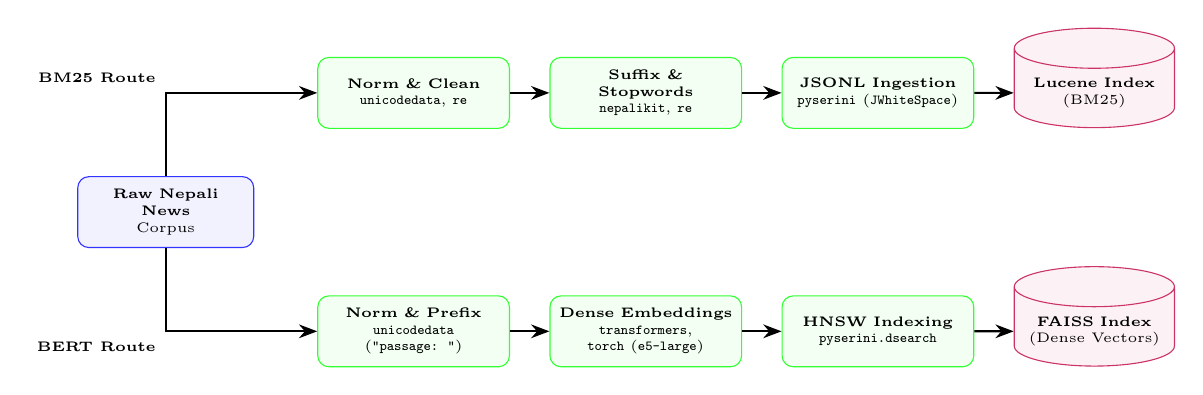
\begin{tikzpicture}[node distance=0.6cm and 0.5cm, >=Stealth, font=\tiny]
    \tikzstyle{block} = [rectangle, draw=blue!80, fill=blue!5, text width=2.0cm, text centered, rounded corners, minimum height=0.9cm]
    \tikzstyle{proc} = [rectangle, draw=green!80, fill=green!5, text width=2.2cm, text centered, rounded corners, minimum height=0.9cm]
    \tikzstyle{db} = [cylinder, draw=purple!80, fill=purple!5, shape border rotate=90, aspect=0.25, text width=1.8cm, text centered, minimum height=0.9cm]

    % Input
    \node [block] (input) {\textbf{Raw Nepali News}\\ Corpus};

    % Top Branch (BM25 Route)
    \node [proc, above right=0.6cm and 0.8cm of input] (bm25_norm) {\textbf{Norm \& Clean}\\ \texttt{unicodedata}, \texttt{re}};
    \node [proc, right=0.5cm of bm25_norm] (bm25_stem) {\textbf{Suffix \& Stopwords}\\ \texttt{nepalikit}, \texttt{re}};
    \node [proc, right=0.5cm of bm25_stem] (bm25_pyserini) {\textbf{JSONL Ingestion}\\ \texttt{pyserini} (\texttt{JWhiteSpace})};
    \node [db, right=0.5cm of bm25_pyserini] (lucene_db) {\textbf{Lucene Index}\\ (BM25)};

    % Bottom Branch (Dense Route)
    \node [proc, below right=0.6cm and 0.8cm of input] (dense_norm) {\textbf{Norm \& Prefix}\\ \texttt{unicodedata} (\texttt{"passage: "})};
    \node [proc, right=0.5cm of dense_norm] (dense_emb) {\textbf{Dense Embeddings}\\ \texttt{transformers}, \texttt{torch} (\texttt{e5-large})};
    \node [proc, right=0.5cm of dense_emb] (dense_pyserini) {\textbf{HNSW Indexing}\\ \texttt{pyserini.dsearch}};
    \node [db, right=0.5cm of dense_pyserini] (faiss_db) {\textbf{FAISS Index}\\ (Dense Vectors)};

    % Connections
    \draw [->, thick] (input) |- node[above left, font=\tiny\bfseries]{BM25 Route} (bm25_norm);
    \draw [->, thick] (bm25_norm) -- (bm25_stem);
    \draw [->, thick] (bm25_stem) -- (bm25_pyserini);
    \draw [->, thick] (bm25_pyserini) -- (lucene_db);

    \draw [->, thick] (input) |- node[below left, font=\tiny\bfseries]{BERT Route} (dense_norm);
    \draw [->, thick] (dense_norm) -- (dense_emb);
    \draw [->, thick] (dense_emb) -- (dense_pyserini);
    \draw [->, thick] (dense_pyserini) -- (faiss_db);
  \end{tikzpicture}
  }
\end{frame}

% Slide 13: Online Inference Pipeline Diagram
\begin{frame}{Online Inference Pipeline}
  \centering
  \resizebox{0.95\textwidth}{!}{
  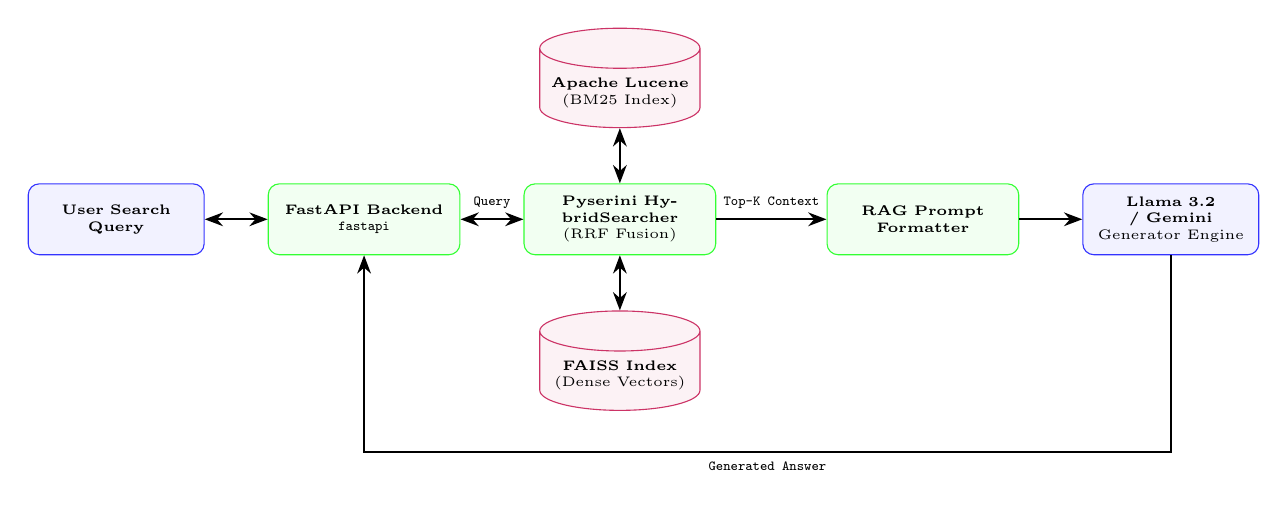
\begin{tikzpicture}[node distance=0.8cm and 0.8cm, >=Stealth, font=\tiny]
    \tikzstyle{block} = [rectangle, draw=blue!80, fill=blue!5, text width=2.0cm, text centered, rounded corners, minimum height=0.9cm]
    \tikzstyle{proc} = [rectangle, draw=green!80, fill=green!5, text width=2.2cm, text centered, rounded corners, minimum height=0.9cm]
    \tikzstyle{db} = [cylinder, draw=purple!80, fill=purple!5, shape border rotate=90, aspect=0.25, text width=1.8cm, text centered, minimum height=0.9cm]

    % Nodes
    \node [block] (q) {\textbf{User Search Query}};
    \node [proc, right=0.8cm of q] (api) {\textbf{FastAPI Backend}\\ \texttt{fastapi}};
    \node [proc, right=0.8cm of api] (hybrid) {\textbf{Pyserini HybridSearcher}\\ (RRF Fusion)};
    
    \node [db, above=0.7cm of hybrid] (lucene) {\textbf{Apache Lucene}\\ (BM25 Index)};
    \node [db, below=0.7cm of hybrid] (faiss) {\textbf{FAISS Index}\\ (Dense Vectors)};

    \node [proc, right=1.4cm of hybrid] (rag) {\textbf{RAG Prompt Formatter}};
    \node [block, right=0.8cm of rag] (llm) {\textbf{Llama 3.2 / Gemini}\\ Generator Engine};

    % Connections
    \draw [<->, thick] (q) -- (api);
    \draw [<->, thick] (api) -- node[above]{\texttt{Query}} (hybrid);
    \draw [<->, thick] (hybrid) -- (lucene);
    \draw [<->, thick] (hybrid) -- (faiss);
    \draw [->, thick] (hybrid) -- node[above]{\texttt{Top-K Context}} (rag);
    \draw [->, thick] (rag) -- (llm);
    \draw [->, thick] (llm.south) -- ++(0,-2.5) -| node[pos=0.25, below, font=\tiny\bfseries]{\texttt{Generated Answer}} (api.south);
  \end{tikzpicture}
  }
\end{frame}

% Slide 14: Tech Stack
\section{Tech Stack}
\begin{frame}{Complete Technology Stack}
  \begin{table}
    \centering
    \begin{tabular}{ll}
      \toprule
      \textbf{Layer} & \textbf{Selected Technologies \& Libraries} \\
      \midrule
      \textbf{Frontend} & React.js, Tailwind CSS \\
      \textbf{Backend API} & FastAPI, Uvicorn \\
      \textbf{IR Framework} & Pyserini, Apache Lucene (\texttt{OpenJDK 11+}) \\
      \textbf{Vector Database} & FAISS (\texttt{faiss-cpu}) \\
      \textbf{Neural Embedder} & \texttt{transformers}, \texttt{torch}, \texttt{intfloat/multilingual-e5-large} \\
      \textbf{Preprocessing} & Python \texttt{unicodedata}, \texttt{re}, \texttt{nepalikit} \\
      \textbf{RAG Generator} & \texttt{meta-llama/Llama-3.2-3B-Instruct} / Google Gemini Flash API \\
      \bottomrule
    \end{tabular}
  \end{table}
\end{frame}

% Slide 15: Future Roadmap - Implicit Feedback & Automatic Data Collection
\begin{frame}{Future Roadmap: Implicit Feedback \& Automated Data Collection}
  \begin{columns}
    \column{0.52\textwidth}
    \begin{block}{Implicit Data Collection Features}
      \begin{itemize}
        \item \textbf{Clickthrough Tracking:} Log user queries alongside the clicked document ID and its result rank position.
        \item \textbf{Dwell Time Logging:} Track time spent reading an article to differentiate true relevance from accidental clicks.
        \item \textbf{Automated $qrels$ Generation:} Map user click patterns directly into query-relevance pairs to auto-expand benchmark datasets.
      \end{itemize}
    \end{block}

    \column{0.48\textwidth}
    \begin{alertblock}{Disclaimer \& Development Context}
      \small
      \textbf{Note:} These implicit feedback mechanisms have \textbf{not been heavily researched} during this initial phase. 
      \vspace{0.2cm}
      
      However, they represent a critical next step for automatically gathering real-world user interaction data to continuously fine-tune and improve search quality for Nepali text.
    \end{alertblock}
  \end{columns}
\end{frame}

% Slide 16: Thank You
\begin{frame}
  \centering
  \Huge \textbf{Thank You!} \\
  \vspace{0.5cm}
  \Large Questions \& Feedback
\end{frame}

\end{document}